%!TEX program = xelatex
% Encoding: UTF8
% SEIKA 2015

%\documentclass[a4paper,11pt,twoside]{book}
\documentclass[letterpaper,11pt,twoside]{ctexbook}

\usepackage{geometry}
\geometry{left=3.5cm, right=3cm, top=3cm, bottom=3cm}
%控制页眉页脚页码
\pagestyle{headings}
%罗马字符页码
%\pagenumbering{roman}

% \usepackage{ctex}
% \usepackage{xeCJK}

%\CJKsetecglue{} % 禁用汉字与其他内容之间空格(空隙)

% 支持西文字体
\usepackage{fourier}
% \usepackage{courier}
% \usepackage{fontspec}

% \newfontfamily\CodeFont{Ubuntu Mono}
\newfontfamily\CodeFont{Consolas}
% \newfontfamily\CodeFont{Lucida Console}
% \setmonofont{Lucida Console}

\usepackage{graphicx}
% 支持插入eps图形文件
% \usepackage{epsfig}

% 支持超链接
\usepackage[colorlinks]{hyperref}

% 支持代码框插入
\usepackage{xcolor}
\definecolor{mygreen}{rgb}{0,0.6,0}
\definecolor{mygray}{rgb}{0.5,0.5,0.5}
\definecolor{mymauve}{rgb}{0.58,0,0.82}
\definecolor{myback}{rgb}{0.95,0.92,0.93}

\usepackage{amsmath}

\usepackage{listings}
\lstset{ %
  backgroundcolor=\color{myback},    % choose the background color; you must add \usepackage{color} or \usepackage{xcolor}
  basicstyle=\linespread{0.95}\footnotesize\CodeFont,   % the size of the fonts that are used for the code
  breakatwhitespace=false,           % sets if automatic breaks should only happen at whitespace
  breaklines=true,                   % sets automatic line breaking
  captionpos=bl,                     % sets the caption-position to bottom
  commentstyle=\color{mygreen},      % comment style
  deletekeywords={...},              % if you want to delete keywords from the given language
  escapeinside={\%*}{*)},            % if you want to add LaTeX within your code
  extendedchars=true,                % lets you use non-ASCII characters; for 8-bits encodings only, does not work with UTF-8
  frame=single,                      % adds a frame around the code
  frameround=tttt,
  keepspaces=true,                   % keeps spaces in text, useful for keeping indentation of code (possibly needs columns=flexible)
  keywordstyle=\color{blue},         % keyword style
  language=Python,                   % the language of the code
  morekeywords={*,...},              % if you want to add more keywords to the set
  numbers=left,                      % where to put the line-numbers; possible values are (none, left, right)
  numbersep=4pt,                     % how far the line-numbers are from the code
  numberstyle=\tiny\CodeFont\color{mygray},   % the style that is used for the line-numbers
  rulecolor=\color{mygray},          % if not set, the frame-color may be changed on line-breaks within not-black text (e.g. comments (green here))
  showspaces=false,                  % show spaces everywhere adding particular underscores; it overrides 'showstringspaces'
  showstringspaces=true,             % underline spaces within strings only
  showtabs=true,                     % show tabs within strings adding particular underscores
  stepnumber=1,                      % the step between two line-numbers. If it's 1, each line will be numbered
  stringstyle=\color{orange},        % string literal style
  tabsize=2,                         % sets default tabsize to 2 spaces
  %title=myPython.py                 % show the filename of files included with \lstinputlisting; also try caption instead of title
  xleftmargin = 2em,
  xrightmargin = 2em,
  aboveskip = 0.5 em
}

% \setCJKmainfont[BoldFont={SimSun},ItalicFont={KaiTi}] %{SimSun}

%%%%%%%%%%%%
\title{Learning Spark }
\author{Holden Karau, Andy Konwinski, Patrick Wendell & matei Zaharia}
\date{\today}
% \thanks{}

\begin{document}

\maketitle
\tableofcontents

%%%% 第一章
\newpage


Ⓔ \textcolor{etc}{This chapter provides a high-level overview of what Apache Spark is. If you are already familiar with Apache Spark and its components, feel free to jump ahead to Chapter 2.}

Ⓒ 本章从顶层概述什么是Apach Spark。如果你已很熟悉 Aparch Spark
及其组件,请跳过此章前往第二章。


%   A NEW SECTION
%%
\section{What is Apache Spark  |  什么是 Apache Spark}\label{whatis_apache_spark}

Ⓔ \textcolor{etc}{Apache Spark is a cluster computing platform designed to be
\emph{fast} and \emph{general purpose}.}

Ⓒ Apache Spark
是一个为\emph{快速}和\emph{通用}性能所设计的集群计算平台。

Ⓔ \textcolor{etc}{On the speed side, Spark extends the popular MapReduce model to efficiently support more types of computations, including interactive queries and stream processing. Speed is important in processing large datasets, as it means the difference between exploring data interactively and waiting minutes or hours. One of the main features Spark offers for speed is the ability to run computations in memory, but the system is also more efficient than MapReduce for complex applications running on disk.}

Ⓒ 就运算速度而言, Spark 延续了流行的 MapReduce 模型从而有效的支援多类计算,包括交互式查询(interactive queries)和流式计算(stream processing)。计算速度对于处理大型数据而言极其重要,在交互式数据探究中等上一分钟或一小时意味着截然不同的分析结果。 Spark最主要的特征之一就是可以在内存中进行计算,同时对于一些更为复杂需要依赖磁盘读写的应用程序,这个系统也能提供优于
MapReduce 的性能。

Ⓔ \textcolor{etc}{On the generality side, Spark is designed to cover a wide range of workloads that previously required separate distributed systems, including batch applications, iterative algorithms, interactive queries, and streaming. By supporting these workloads in the same engine, Spark makes it easy and inexpensive to combine different processing types, which is often necessary in production data analysis pipelines. In addition, it reduces the management burden of maintaining separate tools.}

Ⓒ 就通用性而言, Spark 在设计之初考虑到了现已有的各类分布式系统的任务需求,如 batch applications,迭代算法 (iterative algorithm) ,交互式查询 (interactive queries) ,以及流式计算 (streaming) 。在同一引擎下支持这些不同的任务,Spark可以简单且经济的 \emph{组装} 数据分析生产过程中常用的各类处理类型。此外,Spark减轻了同时维护不同的运维工具所造成管理上的负担。

Ⓔ \textcolor{etc}{Spark is designed to be highly accessible, offering simple APIs in Python, Java, Scala, and SQL, and rich built-in libraries. It also integrates closely with other Big Data tools. In particular, Spark can run in Hadoop clusters and access any Hadoop data source, including Cassandra.}

Ⓒ Spark 在设计上也考虑到了高度可被访问性,提供了简洁的API接口,支持Python,Java,Scala,SQL这些语言,具备丰富的内建库。同时也整合了其他大数据工具。例如,Spark可以在Hadoop集群上运行并且访问任何如Cassandra这样的Hadoop数据源。


%   A NEW SECTION
%%
\section{A unified Stack  |  统一的堆栈}\label{ux7edfux4e00ux7684ux5806ux6808-a-unified-stack}

Ⓔ \textcolor{etc}{The Spark project contains multiple closely integrated components. At its core, Spark is a “computational engine” that is responsible for scheduling, distributing, and monitoring applications consisting of many computational tasks across many worker machines, or a \emph{computing cluster}. Because the core engine of Spark is both fast and general-purpose, it powers multiple higher-level components specialized for various workloads, such as SQL or machine learning. These components are designed to interoperate closely, letting you combine them like libraries in a software project.}

Ⓒ Spark 项目包含了多个相互密切整合的组件。Spark的核心是一个 “计算引擎”负责计划、分发、监视多台工作机器(或称为\emph{计算集群})上执行的计算任务。因为Spark的核心引擎既能高速运算也兼顾通用性,它驱动了多种上层专用任务的组件,如:SQL或机器学习。这些组件在设计上可以紧密的相互操作,让用户感到像软件项目中的库一样便利的将它们结合起来使用。

Ⓔ \textcolor{etc}{A philosophy of tight integration has several benefits. First, all libraries and higher-level components in the stack benefit from improvements at the lower layers. For example, when Spark's core engine adds an optimization, SQL and machine learning libraries automatically speed up as well. Second, the costs associated with running the stack are minimized, because instead of running 5--10 independent software systems, an organization needs to run only one. These costs include deployment, maintenance, testing, support, and others. This also means that each time a new component is added to the Spark stack, every organization that uses Spark will immediately be able to try this new component. This changes the cost of trying out a new type of data analysis from downloading, deploying, and learning a new software project to upgrading Spark.}

Ⓒ 紧密整合的设计哲学带了很多好处。 首先,所有的库和堆栈中高层的组件将得益于低层的改善。比如,当Spark的核心引擎被加入一项优化,SQL 和机器学习库也会自动提高运算性能。 其次,堆栈运行所需要的代价已被最小化,不同于同时运行5--10个独立的软件系统,用户只需要部署和运行一个软件系统即可。这里的代价包括了系统部署、维护、测试、支持和其他方面的成本。这意味着每次新添一个组件到Spark的堆栈,Spark 的用户可以立即试用新装的组件。这就将试验一种新数据分析方式的代价从下载、部署、学习一个新软件变为更新Spark即可。

Ⓔ \textcolor{etc} {Finally, one of the largest advantages of tight integration is the ability to build applications that seamlessly combine different
processing models. For example, in Spark you can write one application that uses machine learning to classify data in real time as it is
ingested from streaming sources. Simultaneously, analysts can query the resulting data, also in real time, via SQL (e.g., to join the data with
unstructured log files). In addition, more sophisticated data engineers and data scientists can access the same data via the Python shell for ad
hoc analysis. Others might access the data in standalone batch applications. All the while, the IT team has to maintain only one system.}

Ⓒ 最终,紧密整合的最大好处在于无缝整合不同处理模型的可能。例如,你可以在Spark中从源代码写一个使用机器学习的进行实时分类的模型。同时别的分析师能够实时的通过诸如SQL的方式(如,用非结构化数据结合查询数据)查询结果数据。此外,资深数据工程师和数据科学家可以通过 Python shell for ad hoc analysis 访问相同的数据。而与此同时,IT团队正在同一个系统上进行着运维。

Ⓔ \textcolor{etc}{Here we will briefly introduce each of Spark's components, shown in Figure 1-1.}

Ⓒ 在此图1-1简明的列出了Spark的各个组件。

\begin{figure}[htbp]
\centering
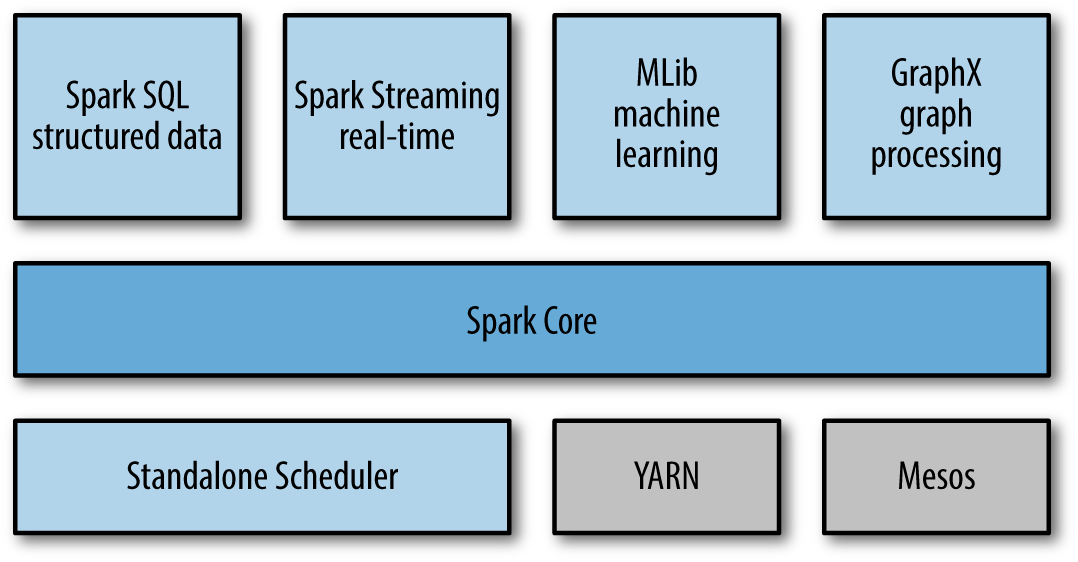
\includegraphics[width=.6\textwidth]{../images/fig_1-1.png}
\caption{The Spark stack  |  Spark堆栈}
\end{figure}

\subsection{Spark 核心组件 (Spark Core)}\label{spark-core}

Ⓔ \textcolor{etc}{Spark Core contains the basic functionality of Spark, including components for task scheduling, memory management, fault recovery, interacting with storage systems, and more. Spark Core is also home to the API that defines resilient distributed datasets (RDDs), which are Spark's main programming abstraction. RDDs represent a collection of items distributed across many compute nodes that can be manipulated in parallel. Spark Core provides many APIs for building and manipulating these collections.}

Ⓒ Spark 核心组件涵盖了Spark的所有基本功能,包括任务计划组件、内存管理、错误还原、与存储系统交互等。Spark核心组件也包含了一个它最主要的编程抽象概念------\emph{弹性分布式数据集}(\emph{resilient distributed datasets}, RDDs),RDDs表示了一个可被并行操作的分布式计算节点的集合。Spark 核心组件提供了很多 API 用于建立和操纵这些集合。

\subsection{Spark SQL}\label{spark-sql}

Ⓔ \textcolor{etc}{Spark SQL is Spark's package for working with structured data. It allows querying data via SQL as well as the Apache Hive variant of SQL---called the Hive Query Language (HQL)---and it supports many sources of data, including Hive tables, Parquet, and JSON. Beyond providing a SQL interface to Spark, Spark SQL allows developers to intermix SQL queries with the programmatic data manipulations supported by RDDs in Python, Java, and Scala, all within a single application, thus combining SQL with complex analytics. This tight integration with the rich computing environment provided by Spark makes Spark SQL unlike any other open source data warehouse tool. Spark SQL was added to Spark in version 1.0.}

Ⓒ Spark~SQL 是 Spark 处理结构化数据的包。它使用SQL或Apache Hive变种的SQL(又被称为Hive查询语言,HQL)语句是查询数据,同时它也支持多种来源的数据,诸如 Hive tables、 Parquet 和 JSON。除了提供连接Spark的SQL接口,Spark SQL让开发者能够在 SQL 查询语句中加入Python、Java 、Scala编写的支持RDD的操控数据的程序,结合简单的应用程序,便使得SQL具备处理复杂分析任务的能力。Spark提供的这种和rich计算环境紧密的结合使Spark SQL与众不同于其他开源数据仓库工具。在Spark 1.0版本后Spark SQL被加入。

Ⓔ \textcolor{etc}{Shark was an older SQL-on-Spark project out of the University of California, Berkeley, that modified Apache Hive to run on Spark. It has now been replaced by Spark SQL to provide better integration with the Spark engine and language APIs.}

Ⓒ Shark 是 Spark 上支持 SQL 的早起开发计划,通过修改 Apache Hive 在Spark上运行,加州大学伯克利分校当时并未参与到此计划。目前它已经被 Spark SQL 这个能与Spark引擎和API更好整合的项目替代。

\subsection{Spark Streaming}\label{spark-streaming}

Ⓔ \textcolor{etc}{Spark Streaming is a Spark component that enables processing of live streams of data. Examples of data streams include log files generated by production web servers, or queues of messages containing status updates posted by users of a web service. Spark Streaming provides an API for manipulating data streams that closely matches the Spark Core's RDD API, making it easy for programmers to learn the project and move between applications that manipulate data stored in memory, on disk, or arriving in real time. Underneath its API, Spark Streaming was designed to provide the same degree of fault tolerance, throughput, and scalability as Spark Core.}

Ⓒ Spark 流式计算 (Spark Streaming) 是 Spark 中运行数据流实时处理的组件。比如由 web 服务器产生的的日志文件,或用户向 web 务器查询的包含状态更新的反馈信息。Spark 流提供了用于操纵数据的与Spark 核心 RDD 高度匹配的API,使得程序员轻而易举的掌握项目从而使得应用对数据的操作在内存、硬盘和实时流处理之间游刃有余。API的下层,Spark 流式计算被设计为提供与上层需求相应程度的错误容忍度、吞吐能力和可扩展性。

\subsection{Spark MLlib  |  Spark 机器学习库 (MLlib)}\label{spark-mllib}

Ⓔ \textcolor{etc}{Spark comes with a library containing common machine learning (ML) functionality, called MLlib. MLlib provides multiple types of machine learning algorithms, including classification, regression, clustering, and collaborative filtering, as well as supporting functionality such as model evaluation and data import. It also provides some lower-level ML primitives, including a generic gradient descent optimization algorithm. All of these methods are designed to scale out across a cluster.}

Ⓒ Sparkz自带了一个包含通用的机器学习(machine learning)功能的库,称作MLlib。 MLlib 提供了多种类型的机器学习算法,包含分类、回归、聚类、以及协作过滤,它也提供了诸如模型评估和数据导入的功能。MLlib同时还支持一些底层的机器学习算法元,例如通用的梯度下降优化法。所有这些算法模型都是面向集群计算规模而设计的。

\subsection{GraphX}\label{graphx}

Ⓔ \textcolor{etc}{GraphX is a library for manipulating graphs (e.g., a social network's friend graph) and performing graph-parallel computations. Like Spark Streaming and Spark SQL, GraphX extends the Spark RDD API, allowing us to create a directed graph with arbitrary properties attached to each vertex and edge. GraphX also provides various operators for manipulating graphs (e.g., subgraph and mapVertices ) and a library of common graph algorithms (e.g., PageRank and triangle counting).}

Ⓒ GraphX 是负责绘制图形(例如朋友圈的社交网络图)的库件,同时还能进行图的并行演算。和Spark流式计算和Spark SQL一样,它延伸的Spark RDD的API,从而让我们能直接建立顶点和边带有任意属性注释的图表。GraphX同时提供了丰富的操作方式用于调节图表显示(如图集嵌套和顶点映射)和包含通用的图形模板(如页面排序和三角形计数)的库。

\subsection{Cluster Managers  |  集群管理器}\label{cluster-managers}

Ⓔ \textcolor{etc}{Under the hood, Spark is designed to efficiently scale up from one to many thousands of compute nodes. To achieve this while maximizing flexibility, Spark can run over a variety of cluster managers, including Hadoop YARN, Apache Mesos, and a simple cluster manager included in Spark itself called the Standalone Scheduler. If you are just installing Spark on an empty set of machines, the Standalone Scheduler provides an easy way to get started; if you already have a Hadoop YARN or Mesos cluster, however, Spark's support for these cluster managers allows your applications to also run on them. Chapter 7 explores the different options and how to choose the correct cluster manager.}

Ⓒ 在底层,Saprk设计时考虑到了能从一个计算节点扩大到数千个的能力。同时为了最大的满足其灵活性,Spark 可以在很多集群管理器之下运行,包括 Hadoop YARN、Apache Mesos 以及像Spark本身那个样的单点集群管理器(被称作 Standalone Scheduler)。如果您在一台新机器上安装Spark,Standalone Scheduler 会提供简单的方式让您上手;如果您已经拥有了Hadoop YARN 或者 Mesos 集群,Spark 依然可以支持这些集群,在其上运行你的Spark应用。第7章我们会详细介绍选择不同集群管理器的区别。

\section{Spark的使用者和使用目的 Who Uses Spark, and for What?}\label{spark-who-uses-spark-and-for-what}

Ⓔ \textcolor{etc}{Because Spark is a general-purpose framework for cluster computing, it is used for a diverse range of applications. In the Preface we outlined two groups of readers that this book targets: data scientists and engineers. Let's take a closer look at each group and how it uses Spark. Unsurprisingly, the typical use cases differ between the two, but we can roughly classify them into two categories, data science and data applications.}

Ⓒ 因为Spark是一个为通用目的开发的集群管理框架,它可被用于许多不同的应用场景。在序章中我们列出了本书的两类目标读者人群:数据科学家和数据工程师。我们现在仔细探讨一下两类人群是如何使用Spark的。不出意外,两者之间的使用案例典型各不相同,故而我们可以粗略的将案例分为两类:数据科学和数据应用。

Ⓔ \textcolor{etc}{Of course, these are imprecise disciplines and usage patterns, and many folks have skills from both, sometimes playing the role of the investigating data scientist, and then "changing hats" and writing a hardened data processing application. Nonetheless, it can be illuminating to consider the two groups and their respective use cases separately.}

Ⓒ 当然这也不是精确学科和使用模式的划分,很多用户对两方面都很精通,有的人既可以在数据探究时扮演数据科学家的角色,也能迅速转换角色写出过硬的数据处理应用。尽管如此,明晰两种人群所负责的不同职能也是也能有必要的。

\subsection{数据科学家的任务 Data Science Tasks}\label{data-science-tasks}

Ⓔ \textcolor{etc}{Data science, a discipline that has been emerging over the past few years, centers on analyzing data. While there is no standard definition, for our purposes a data scientist is somebody whose main task is to analyze and model data. Data scientists may have experience with SQL, statistics, predictive modeling (machine learning), and programming, usually in Python, Matlab, or R. Data scientists also have experience with techniques necessary to transform data into formats that can be analyzed for insights (sometimes referred to as data wrangling).}

Ⓒ 数据科学是,一门过去几年刚刚涌现的学科,着眼于分析数据的学科。尽管对其尚未形成标准的定义,我们说定义的数据科学家其主要职责是对数据分析并建模。数据科学家应该具备使用SQL、统计学、预测模型(如机器学习)、编程语言(如Python、Matlab或者R)的经验能力。同时他们应具备必要的技能把数据转换成他们所需分析的形式,这种工作通常也被称为 data wrangling。

Ⓔ \textcolor{etc}{Data scientists use their skills to analyze data with the goal of answering a question or discovering insights. Oftentimes, their workflow involves ad hoc analysis, so they use interactive shells (versus building complex applications) that let them see results of queries and snippets of code in the least amount of time. Spark's speed and simple APIs shine for this purpose, and its built-in libraries mean that many algorithms are available out of the box.}

Ⓒ 数据科学家使用他们的技能分析研究数据从而回答一些问题或能洞察未知的知识。他们通常的工作流程包含了非既定的数据探究分析,一次他们需要使用交互的分析界面(相对于写一个复杂的应用)好让他们在最快时间内看到查询或代码片段的分析结果。Spark的快速简介的API正是为此而来,同时它的内建库已经具备大量现成可用的算法。

Ⓔ \textcolor{etc}{Spark supports the different tasks of data science with a number of components. The Spark shell makes it easy to do interactive data analysis using Python or Scala. Spark SQL also has a separate SQL shell that can be used to do data exploration using SQL, or Spark SQL can be used as part of a regular Spark program or in the Spark shell. Machine learning and data analysis is supported through the MLLib libraries. In addition, there is support for calling out to external programs in Matlab or R. Spark enables data scientists to tackle problems with larger data sizes than they could before with tools like R or Pandas.}

Ⓒ Spark的很多组件支持数据科学研究的不同任务。Spark shell允许使用Python或Scala语言就可以轻易的实现交互式数据分析。Spark SQL也具备一个独立的SQL shell,它能支持使用SQL或Spark SQL进行数据探究,这些代码可以被应用到标准的标准Spark程序中或是直接在Spark shell中调试。MLLib是支持机器学习和数据分析的库。此外,Spark也可以被外部程序如Matlab或R调用。因此,数据现在科学家可以使用Spark轻松处理那些在R或Pandas中无法胜任的求解大规模数据的问题。

Ⓔ \textcolor{etc}{Sometimes, after the initial exploration phase, the work of a data scientist will be "productized", or extended, hardened (i.e., made fault-tolerant), and tuned to become a production data processing application, which itself is a component of a business application. For example, the initial investigation of a data scientist might lead to the creation of a production recommender system that is integrated into a web application and used to generate product suggestions to users. Often it is a different person or team that leads the process of productizing the work of the data scientists, and that person is often an engineer.}

Ⓒ 通常,初步的探究阶段完成之后,数据科学家们的任务就是将研究``产品化'',抑或是扩展化、固化(也就是说增加容错性),使之成为一个商业应用的一个组件,能够处理数据的应用的产品。例如,一个数据科学家初步探研可能最终演化为一个可整合到web应用的推荐系统,用于推测可向用户推荐的产品。通常会由其他研发人员或团队将数据科学家的工作产品化,他们就是数据工程师。

\subsection{数据处理应用 Data Processing Applications} \label{data-processing-applications}

Ⓔ \textcolor{etc}{The other main use case of Spark can be described in the context of the engineer persona. For our purposes here, we think of engineers as a large class of software developers who use Spark to build production data processing applications. These developers usually have an understanding of the principles of software engineering, such as encapsulation, interface design, and object-oriented programming. They frequently have a degree in computer science. They use their engineering skills to design and build software systems that implement a business use case.}

Ⓒ Spark的另一主要使用群体是数据工程师。在此,我们考虑了到工程师们作为软件开发人员的主体,使用Spark构建数据处理应用。这些开发者们往往深谙软件工程开发之路,如封装、界面设计、面向对象编程。他们往往是计算机科学专业科班出身,能够使用软件工程开发技术设计并开发软件系统重而实现特定的商业用途。

Ⓔ \textcolor{etc}{For engineers, Spark provides a simple way to parallelize these applications across clusters, and hides the complexity of distributed systems programming, network communication, and fault tolerance. The system gives them enough control to monitor, inspect, and tune applications while allowing them to implement common tasks quickly. The modular nature of the API (based on passing distributed collections of objects) makes it easy to factor work into reusable libraries and test it locally.}

Ⓒ 对于软件工程师而言,Spark提供了简便的方式实现应用在集群见的并行运算,将复杂的分布式系统编程、网络通信编程、容错机制设计隐藏在后台。系统在快速执行任务的同时给予开发者足够的控制权监视、inspect、调试应用。API模块(基于分散和派发对象)的天然属性简单的把工作变为可复用的库并在本地测试。

Ⓔ \textcolor{etc}{Spark's users choose to use it for their data processing applications because it provides a wide variety of functionality, is easy to learn and use, and is mature and reliable.}

Ⓒ 用户之所以选择Spark来进行数据处理和开发是应为它功能上提供了宽泛的可变性,易于学习和使用,是成熟可靠的技术。

\section{A Brief History of Spark  |  Spark简史}\label{a-brief-history-of-spark}

Ⓔ \textcolor{etc}{Spark is an open source project that has been built and is maintained by a thriving and diverse community of developers. If you or your organization are trying Spark for the first time, you might be interested in the history of the project. Spark started in 2009 as a research project in the UC Berkeley RAD Lab, later to become the AMPLab. The researchers in the lab had previously been working on Hadoop MapReduce, and observed that MapReduce was inefficient for iterative and interactive computing jobs. Thus, from the beginning, Spark was designed to be fast for interactive queries and iterative algorithms, bringing in ideas like support for in-memory storage and efficient fault recovery.}

Ⓒ Spark 是由thriving和diverse的开发者社区开发并维护的开源项目。如果您或您的机构已在第一时间试用了Spark,可能您也会对该项目的历史有点兴趣。作为加州大学伯克利分校RAD实验室以及后来的AMPLab实验室的一个研究项目,Spark项目于2009年启动。实验室的研究者之前也参与了Hadoop MapReduce项目,并意识到MapReduce对于迭代和交互式计算任务的低效性。因此,Spark设计之初就考虑到高速的交互式查询和迭代算法的运算,创造出了支持在内存存储计算和高效的容错恢复机制。

Ⓔ \textcolor{etc}{Research papers were published about Spark at academic conferences and soon after its creation in 2009, it was already 10--20$\times$ faster than MapReduce for certain jobs.}

Ⓒ 关于Spark的研究论文很快于2009年在学术会议中发表,当时已经达到了处理日常任务时快于MapReduce10--20倍。

Ⓔ \textcolor{etc}{Some of Spark's first users were other groups inside UC Berkeley, including machine learning researchers such as the Mobile Millennium project, which used Spark to monitor and predict traffic congestion in the San Francisco Bay Area. In a very short time, however, many external organizations began using Spark, and today, over 50 organizations list themselves on the Spark PoweredBy page, and dozens speak about their use cases at Spark community events such as Spark Meetups and the Spark Summit. In addition to UC Berkeley, major contributors to Spark include Databricks, Yahoo!, and Intel.}

Ⓒ Spark的第一批使用者时UC伯克利大学的其它小组,包括了机器学习的研究者,如Mobile Millennium Project,他们使用Spark监视并预测三藩市湾岸地区的交通拥堵现象。然而很快,大量外部机构开始使用Spark,到目前为止,约有50个组织将它们列在Spark支持主页上,并在很多Spark社区活动(如Spark碰头会或Spark峰会)上分享宣讲了他们使用Spark的案例。此外,除了加州伯克利大学,Databricks、Yahoo!和Intel也成为Spark的主要贡献者。

Ⓔ \textcolor{etc}{In 2011, the AMPLab started to develop higher-level components on Spark, such as Shark (Hive on Spark) 1 and Spark Streaming. These and other components are sometimes referred to as the Berkeley Data Analytics Stack (BDAS).}

Ⓒ 2011年,AMPLab实验室着手开发Spark更高一级别的组件,例如 Shark (Hive on Spark) 1 和 Spark Streaming。这类组件有时也被称为伯克利数据分析栈(Berkeley Data Analytics Stack,BDAS)。

Ⓔ \textcolor{etc}{Spark was first open sourced in March 2010, and was transferred to the Apache Software Foundation in June 2013, where it is now a top-level project.}

Ⓒ 2011年3月,Spark项目开始公开源代码,并于2013年6月转入阿帕奇软件基金会(Apache Software Foundation)旗下,至今认为该组织的顶级研发项目。

\section{Spark Versions and Releases  |  Spark的发行版} \label{spark-versions-and-releases}

Ⓔ \textcolor{etc}{Since its creation, Spark has been a very active project and community, with the number of contributors growing with each release. Spark 1.0 had over 100 individual contributors. Though the level of activity has rapidly grown, the community continues to release updated versions of Spark on a regular schedule. Spark 1.0 was released in May 2014. This book focuses primarily on Spark 1.1.0 and beyond, though most of the concepts and examples also work in earlier versions.}

Ⓒ 从创建之初,Spark的项目和其社区一直都很活跃,每次更新中拥有大量贡献者的身影。Spark 1.0 拥有超过100位独立的贡献者。尽管活跃度日益增长,Spark社区保持按照规则的路线图释放更新。Spark 1.0 于2014年5月释出。本书主要以Spark 1.10 及其后续版本为参考,大多数内容概念与示例仍与早期版本兼容。

\section{Storage Layers for Spark  |  Spark的存储层} \label{storage-layers-for-spark}

Ⓔ \textcolor{etc}{Spark can create distributed datasets from any file stored in the Hadoop distributed filesystem (HDFS) or other storage systems supported by the Hadoop APIs (including your local filesystem, Amazon S3, Cassandra, Hive, HBase, etc.). It's important to remember that Spark does not require Hadoop; it simply has support for storage systems implementing the Hadoop APIs. Spark supports text files, SequenceFiles, Avro, Parquet, and any other Hadoop InputFormat. We will look at interacting with these data sources in Chapter 5.}

Ⓒ Spark 可以从任何存储在Hadoop分布文件系统(HDFS)上的文件或是其他Hadoop API 支持的文件系统(包括你的本地文件系统、Amazon S3、Cassandra、Hive、HBase等)建立分布式数据集。需要注意的是,Spark本身并不依赖Hadoop,它已支持存储系统调用Hadoop API。Spark也支持文本文件、序列化文件、Avro、Parquet和一些其他的Hadoop输出格式。 我们将在第五章详细探讨这些数据源的使用。

% \include{get_started/c1s02_os_setup}
% \include{get_started/c1s03_basic_usage}
\end{document}

